% !TeX program = xelatex
\documentclass[aspectratio=169,10pt]{beamer}

% ==================== Theme ====================
\usetheme{Madrid}
\usecolortheme{default}
\setbeamertemplate{navigation symbols}{}
\setbeamertemplate{footline}[frame number]
\setbeameroption{hide notes}

% ==================== Packages ====================
\usepackage{booktabs}
\usepackage{tabularx}
\usepackage{array}
\usepackage{graphicx}
\usepackage{tikz}
\usepackage{amsmath}
\usepackage{hyperref}
\usetikzlibrary{arrows.meta,positioning,fit,calc,shapes.geometric}

% ==================== Colours ====================
\definecolor{DeepGreen}{HTML}{0B5D4B}
\definecolor{AccentGreen}{HTML}{16A085}
\definecolor{WarmRed}{HTML}{C0392B}
\definecolor{Amber}{HTML}{D68910}
\definecolor{Ink}{HTML}{1F2937}
\definecolor{SoftGrey}{HTML}{F3F4F6}
\definecolor{MidGrey}{HTML}{6B7280}
\definecolor{PaleGreen}{HTML}{E8F6F3}
\definecolor{PaleRed}{HTML}{FDEDEC}
\definecolor{PaleAmber}{HTML}{FEF5E7}

\setbeamercolor{title}{fg=DeepGreen}
\setbeamercolor{frametitle}{fg=DeepGreen,bg=SoftGrey}
\setbeamercolor{structure}{fg=DeepGreen}
\setbeamercolor{block title}{fg=white,bg=DeepGreen}
\setbeamercolor{block body}{fg=Ink,bg=SoftGrey}
\setbeamercolor{alerted text}{fg=WarmRed}

% ==================== Helpers ====================
\newcommand{\metricbox}[3]{%
  \begin{tikzpicture}[baseline]
    \node[rounded corners=3pt, fill=#1, inner xsep=5pt, inner ysep=3pt, text=white, font=\scriptsize\bfseries] {#2: #3};
  \end{tikzpicture}%
}

\newcommand{\smallchip}[2]{%
  \begin{tikzpicture}[baseline]
    \node[rounded corners=3pt, draw=#1, fill=#1!8, inner xsep=4pt, inner ysep=2pt, text=Ink, font=\scriptsize] {#2};
  \end{tikzpicture}%
}

\newcommand{\tick}{\textcolor{DeepGreen}{\textbf{Yes}}}
\newcommand{\cross}{\textcolor{WarmRed}{\textbf{No}}}

\title[LLM Fine-Tuning for T20 Score Prediction]{Context-Aware Fine-Tuning of Large Language Models\\for First-Innings Score Prediction in T20 Cricket}
\subtitle{MSc Viva Presentation}
\author[Damith T. A. R. Ratnayaka]{Damith Tilanka Abewardana Ranasingha Ratnayaka}
\institute[USJ]{University of Sri Jayewardenepura\\Supervisor: Dr. Rajitha M. Silva}
\date{June 2026}

\begin{document}

% =================================================
% Slide 1
% =================================================
\begin{frame}[plain]
  \titlepage
  \vspace{-0.4cm}
  \begin{center}
    \smallchip{DeepGreen}{MSc DSA 055} \hspace{0.4em}
    \smallchip{AccentGreen}{Cricsheet T20I data} \hspace{0.4em}
    \smallchip{Amber}{Llama 3.2-3B + QLoRA}
  \end{center}
  \note{Good morning. My thesis investigates whether a compact open-source LLM, fine-tuned with QLoRA on domain-specific natural-language prompts, can predict T20 first-innings totals competitively from any mid-innings snapshot.}
\end{frame}

% =================================================
% Slide 2
% =================================================
\begin{frame}{Motivation \& Significance}
\begin{columns}[T,onlytextwidth]
  \column{0.48\textwidth}
  \begin{block}{Why T20 score prediction matters}
    \begin{itemize}
      \item Broadcast graphics and live commentary
      \item Fantasy and betting market projections
      \item Tactical planning for batting and bowling units
      \item Short format, high variance, rapidly changing innings state
    \end{itemize}
  \end{block}

  \vspace{0.15cm}
  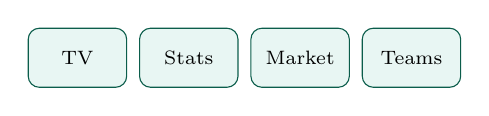
\begin{tikzpicture}[node distance=0.15cm]
    \node[draw=DeepGreen, fill=PaleGreen, rounded corners=4pt, minimum width=1.25cm, minimum height=0.75cm, font=\scriptsize] (a) {TV};
    \node[draw=DeepGreen, fill=PaleGreen, rounded corners=4pt, minimum width=1.25cm, minimum height=0.75cm, font=\scriptsize, right=of a] (b) {Stats};
    \node[draw=DeepGreen, fill=PaleGreen, rounded corners=4pt, minimum width=1.25cm, minimum height=0.75cm, font=\scriptsize, right=of b] (c) {Market};
    \node[draw=DeepGreen, fill=PaleGreen, rounded corners=4pt, minimum width=1.25cm, minimum height=0.75cm, font=\scriptsize, right=of c] (d) {Teams};
  \end{tikzpicture}

  \column{0.48\textwidth}
  \begin{block}{Core opportunity}
    Conventional models usually consume a flat numeric vector:
    \vspace{0.15cm}

    \small\texttt{overs=12, runs=95, wickets=3, par=165}

    \vspace{0.25cm}
    But analysts reason in context-rich language:

    \vspace{0.15cm}
    \small\itshape
    ``95 for 3 after 12 overs, with two strong batters still available, at a 165-par venue.''
  \end{block}
  \vspace{0.15cm}
  \alert{Research premise:} LLMs can exploit this semantic representation after domain-specific fine-tuning.
\end{columns}
\note{T20 is short, high-variance, commercially dominant. A reliable score predictor must integrate batting depth, venue context, recent momentum and phase of play simultaneously.}
\end{frame}

% =================================================
% Slide 3
% =================================================
\begin{frame}{Research Objectives \& Scope}
\scriptsize
\begin{tabularx}{\textwidth}{@{}>{\bfseries}p{0.8cm}X >{\bfseries}p{0.8cm}X@{}}
\toprule
RO1 & Construct T20 snapshot dataset with engineered features including RBSS & RO2 & Design natural-language prompt schema and prompt-completion corpus \\
RO3 & Establish zero-shot Llama 3.2-3B baseline & RO4 & Fine-tune Llama 3.2-3B using QLoRA SFT \\
RO5 & Compare minimum-validation-loss and final checkpoints & RO6 & Evaluate GPT-4.1-nano zero-shot as frontier reference \\
\bottomrule
\end{tabularx}

\vspace{0.5cm}
\begin{columns}[T,onlytextwidth]
  \column{0.49\textwidth}
  \begin{block}{In scope}
    \begin{itemize}
      \item International men's T20 matches
      \item First-innings final score prediction
      \item Two-over in-game snapshots
      \item Parameter-efficient fine-tuning
    \end{itemize}
  \end{block}
  \column{0.49\textwidth}
  \begin{block}{Out of scope}
    \begin{itemize}
      \item Domestic leagues such as IPL, BBL, PSL
      \item Second-innings chase probability
      \item Full-parameter fine-tuning
      \item Multi-seed training analysis
    \end{itemize}
  \end{block}
\end{columns}
\note{The objectives map cleanly to the thesis chapters and define the evaluation contract: data, prompt schema, baselines, fine-tuning, checkpoint comparison and frontier reference.}
\end{frame}

% =================================================
% Slide 4
% =================================================
\begin{frame}{Literature Review (1): Themes \& Trajectory}
\scriptsize
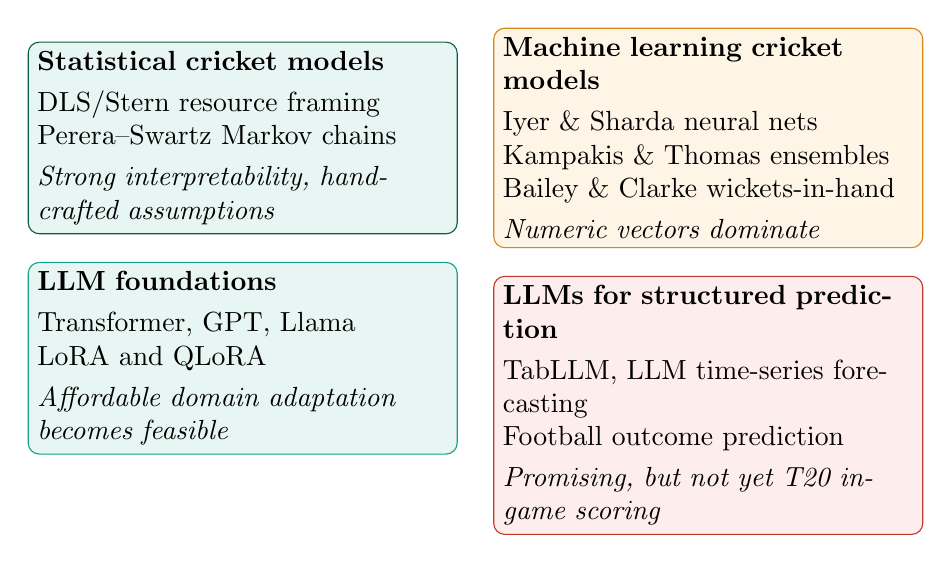
\begin{tikzpicture}[node distance=0.25cm]
  \node[draw=DeepGreen, fill=PaleGreen, rounded corners=4pt, text width=0.43\textwidth, minimum height=2.25cm, align=left] (stat) {
    \textbf{Statistical cricket models}\\[0.1cm]
    DLS/Stern resource framing\\
    Perera--Swartz Markov chains\\[0.1cm]
    \textit{Strong interpretability, hand-crafted assumptions}
  };
  \node[draw=Amber, fill=PaleAmber, rounded corners=4pt, text width=0.43\textwidth, minimum height=2.25cm, align=left, right=0.45cm of stat] (ml) {
    \textbf{Machine learning cricket models}\\[0.1cm]
    Iyer \& Sharda neural nets\\
    Kampakis \& Thomas ensembles\\
    Bailey \& Clarke wickets-in-hand\\[0.1cm]
    \textit{Numeric vectors dominate}
  };
  \node[draw=AccentGreen, fill=PaleGreen, rounded corners=4pt, text width=0.43\textwidth, minimum height=2.25cm, align=left, below=0.35cm of stat] (llm) {
    \textbf{LLM foundations}\\[0.1cm]
    Transformer, GPT, Llama\\
    LoRA and QLoRA\\[0.1cm]
    \textit{Affordable domain adaptation becomes feasible}
  };
  \node[draw=WarmRed, fill=PaleRed, rounded corners=4pt, text width=0.43\textwidth, minimum height=2.25cm, align=left, below=0.35cm of ml] (app) {
    \textbf{LLMs for structured prediction}\\[0.1cm]
    TabLLM, LLM time-series forecasting\\
    Football outcome prediction\\[0.1cm]
    \textit{Promising, but not yet T20 in-game scoring}
  };
\end{tikzpicture}

\vspace{0.25cm}
\centering
\alert{Trajectory:} hand-crafted resources $\rightarrow$ numeric ML $\rightarrow$ language-model structured prediction.
\note{This is a thematic review, not a paper-by-paper recital. The central movement is from explicit statistical assumptions to domain-adapted language models.}
\end{frame}

% =================================================
% Slide 5
% =================================================
\begin{frame}{Literature Review (2): Research Gap \& Contribution Map}
\scriptsize
\renewcommand{\arraystretch}{1.25}
\begin{tabularx}{\textwidth}{@{}lcccc@{}}
\toprule
\textbf{Study / stream} & \textbf{T20 prompt} & \textbf{RBSS-like} & \textbf{Small FT vs frontier} & \textbf{PEFT checkpoint} \\
\midrule
Perera--Swartz / Markov cricket & \cross & \cross & \cross & \cross \\
Kampakis / ML cricket & \cross & \cross & \cross & \cross \\
Hegselmann / TabLLM & \cross & \cross & \cross & \cross \\
Huckerby / LLM football & \cross & \cross & \cross & \cross \\
\rowcolor{PaleGreen}
\textbf{This thesis} & \tick & \tick & \tick & \tick \\
\bottomrule
\end{tabularx}

\vspace{0.45cm}
\begin{block}{Synthesised gap}
No prior work combines a natural-language T20 match-state prompt, RBSS-style batting-depth encoding, QLoRA fine-tuning of a compact open-source LLM, and a head-to-head benchmark against a frontier zero-shot model.
\end{block}
\note{This slide is the novelty defence. The individual building blocks exist elsewhere, but this exact task, representation and comparison protocol are new in cricket analytics.}
\end{frame}

% =================================================
% Slide 6
% =================================================
\begin{frame}{Methodology Overview}
\scriptsize

\begin{tikzpicture}[
  stage/.style={draw=DeepGreen, fill=PaleGreen, rounded corners=4pt, text width=2.05cm, minimum height=1.2cm, align=center, font=\scriptsize\bfseries},
  arrow/.style={-{Latex[length=2mm]}, thick, draw=MidGrey}
]
  \node[stage] (a) {Cricsheet JSON\\3,113 matches};
  \node[stage, right=0.35cm of a] (b) {Filter + venue normalise\\2,895 matches\\236 venues};
  \node[stage, right=0.35cm of b] (c) {Feature engineering\\16 features\\10 snapshots};
  \node[stage, right=0.35cm of c] (d) {Prompt corpus\\28,950 rows\\temporal split};
  \node[stage, right=0.35cm of d] (e) {QLoRA SFT\\Llama 3.2-3B\\step 800};
  \node[stage, right=0.35cm of e] (f) {Evaluation + deployment\\3 conditions};
  \draw[arrow] (a) -- (b);
  \draw[arrow] (b) -- (c);
  \draw[arrow] (c) -- (d);
  \draw[arrow] (d) -- (e);
  \draw[arrow] (e) -- (f);
\end{tikzpicture}

\vspace{0.5cm}
\begin{columns}[T,onlytextwidth]
  \column{0.32\textwidth}
  \begin{block}{Data hygiene}
  No-result and incomplete first innings removed.
  \end{block}
  \column{0.32\textwidth}
  \begin{block}{Leakage control}
  Match-level temporal split before evaluation.
  \end{block}
  \column{0.32\textwidth}
  \begin{block}{Artefacts}
  HF datasets, HF adapter, W\&B logs, Modal service.
  \end{block}
\end{columns}
\note{Everything that follows fits inside this pipeline. The temporal split is the main guardrail against leakage and mirrors a realistic deployment setting.}
\end{frame}

% =================================================
% Slide 7
% =================================================
\begin{frame}{Feature Engineering \& RBSS}
\scriptsize
\begin{columns}[T,onlytextwidth]
  \column{0.48\textwidth}
  \begin{block}{Snapshot construction}
    \begin{itemize}
      \item First innings divided into ten 2-over sections
      \item One prompt-completion pair per section
      \item Feature groups: state, recent momentum, phase, venue, RBSS
      \item Venue par score: 52nd percentile of historical first-innings totals
    \end{itemize}
  \end{block}

  \begin{block}{RBSS definition}
    \[
      \text{RBSS}=\sum_{p\in \mathcal{R}} w(\text{class}(p))
    \]
    $\mathcal{R}$ = undismissed players at the end of the section.
  \end{block}

  \column{0.48\textwidth}
  \renewcommand{\arraystretch}{1.15}
  \begin{tabularx}{\textwidth}{@{}Xr@{}}
  \toprule
  \textbf{Player class} & \textbf{Weight} \\
  \midrule
  Batter & 1.00 \\
  All-rounder & 0.80 \\
  Utility player & 0.65 \\
  Insufficient data & 0.45 \\
  Bowler & 0.30 \\
  \bottomrule
  \end{tabularx}

  \vspace{0.35cm}
  \begin{block}{Worked example}
  \centering
  $1(1.00)+2(0.80)+1(0.65)+3(0.30)=\mathbf{4.15}$
  \end{block}

  \vspace{0.15cm}
  \alert{Why it matters:} identical scorelines can have different remaining batting quality.
\end{columns}
\note{RBSS encodes residual batting quality, not just wickets in hand. This is the most important feature-engineering novelty in the thesis.}
\end{frame}

% =================================================
% Slide 8
% =================================================
\begin{frame}{Prompt Schema \& Model Architecture}
\scriptsize
\begin{columns}[T,onlytextwidth]
  \column{0.47\textwidth}
  \begin{block}{Prompt skeleton}
\ttfamily\scriptsize
Match type: T20\\
Venue: \{venue\}\\
Venue par score: \{par\}\\
Batting team: \{team\}\\[0.1cm]
Overs completed: \{overs\}\\
Balls remaining: \{balls\}\\
Runs scored: \{runs\}\\
Wickets lost: \{wickets\}\\
Current run rate: \{rate\}\\[0.1cm]
Runs in last 2 overs: \{recent\}\\
Dot balls so far: \{dots\}\\
Fours hit: \{fours\} ; Sixes hit: \{sixes\}\\
Powerplay completed: \{Yes/No\}\\
Remaining Batting Strength Score: \{RBSS\}\\
Final 1st innings score:
  \end{block}
  \smallchip{DeepGreen}{max prompt length: 148 tokens} \quad \smallchip{AccentGreen}{max seq length: 256}

  \column{0.50\textwidth}
  \begin{block}{QLoRA fine-tuning recipe}
  \begin{tabularx}{\textwidth}{@{}lX@{}}
  Base model & Llama 3.2-3B decoder-only \\
  Quantisation & 4-bit NF4 + double quantisation \\
  LoRA & $r=16$, $\alpha=32$, dropout 0.1 \\
  Targets & \texttt{q\_proj}, \texttt{k\_proj}, \texttt{v\_proj}, \texttt{o\_proj} \\
  Training & 1 epoch, lr $2\times10^{-4}$ cosine \\
  Hardware & Kaggle NVIDIA T4, fp16, batch eff. 8 \\
  \end{tabularx}
  \end{block}

  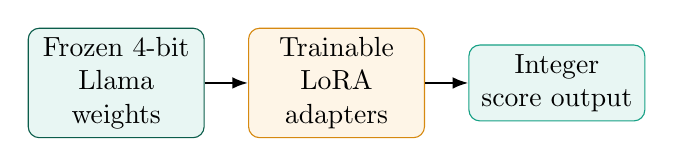
\begin{tikzpicture}[node distance=0.25cm]
    \node[draw=DeepGreen, fill=PaleGreen, rounded corners=4pt, text width=2.0cm, align=center] (base) {Frozen 4-bit\\Llama weights};
    \node[draw=Amber, fill=PaleAmber, rounded corners=4pt, text width=2.0cm, align=center, right=0.55cm of base] (lora) {Trainable\\LoRA adapters};
    \node[draw=AccentGreen, fill=PaleGreen, rounded corners=4pt, text width=2.0cm, align=center, right=0.55cm of lora] (out) {Integer\\score output};
    \draw[-{Latex[length=2mm]}, thick] (base) -- (lora);
    \draw[-{Latex[length=2mm]}, thick] (lora) -- (out);
  \end{tikzpicture}
\end{columns}
\note{The completion is a single integer. The fine-tuning is designed to be reproducible on consumer-grade hardware.}
\end{frame}

% =================================================
% Slide 9
% =================================================
\begin{frame}{Data, Splits \& Tools}
\scriptsize
\begin{columns}[T,onlytextwidth]
  \column{0.52\textwidth}
  \begin{block}{Strict temporal split}
  \renewcommand{\arraystretch}{1.15}
  \begin{tabularx}{\textwidth}{@{}lXrr@{}}
  \toprule
  \textbf{Split} & \textbf{Date range} & \textbf{Matches} & \textbf{Rows} \\
  \midrule
  Train & Up to 2024-12-31 & 2,408 & 24,080 \\
  Validation & 2025-01-01 to 2025-06-30 & 237 & 2,370 \\
  Test & 2025-07-01 onwards & 250 & 2,500 \\
  \bottomrule
  \end{tabularx}
  \end{block}
  \begin{itemize}
    \item Match-level chronological partitioning
    \item Simulates future deployment conditions
    \item Reduces risk of temporal leakage
  \end{itemize}

  \column{0.44\textwidth}
  \begin{block}{Reproducibility stack}
    Pydantic v2, SQLite, fuzzywuzzy, Hugging Face Datasets, PEFT, TRL, BitsAndBytes, W\&B, LiteLLM, Modal, Gradio, React/Vite, Azure Static Web Apps.
  \end{block}
  \vspace{0.25cm}
  \metricbox{DeepGreen}{W\&B run}{v64wpa10}\\[0.15cm]
  \metricbox{AccentGreen}{HF adapter}{00be3f3f}\\[0.15cm]
  \metricbox{Amber}{Dataset}{28,950 rows}
\end{columns}
\note{Two choices are crucial: temporal splitting and artefact pinning. The adapter revision makes the reported model state unambiguous.}
\end{frame}

% =================================================
% Slide 10
% =================================================
\begin{frame}{Results: Fine-Tuned 3B Beats Zero-Shot Frontier}
\scriptsize
\begin{columns}[T,onlytextwidth]
  \column{0.58\textwidth}
  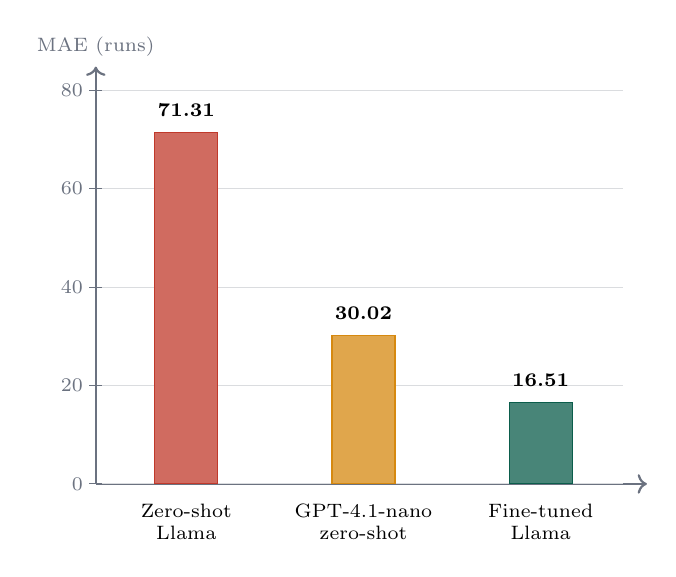
\begin{tikzpicture}
    \draw[->, MidGrey, thick] (0,0) -- (0,5.3) node[above, font=\scriptsize] {MAE (runs)};
    \draw[->, MidGrey, thick] (0,0) -- (7.0,0);
    \foreach \y/\label in {0/0,1.25/20,2.5/40,3.75/60,5.0/80} {
      \draw[MidGrey] (-0.08,\y) -- (0.08,\y) node[left=0.12cm, font=\scriptsize] {\label};
      \draw[MidGrey!25] (0.08,\y) -- (6.7,\y);
    }
    \fill[WarmRed!75, draw=WarmRed] (0.75,0) rectangle (1.55,4.46);
    \fill[Amber!75, draw=Amber] (3.0,0) rectangle (3.8,1.88);
    \fill[DeepGreen!75, draw=DeepGreen] (5.25,0) rectangle (6.05,1.03);
    \node[font=\scriptsize\bfseries] at (1.15,4.75) {71.31};
    \node[font=\scriptsize\bfseries] at (3.40,2.17) {30.02};
    \node[font=\scriptsize\bfseries] at (5.65,1.32) {16.51};
    \node[font=\scriptsize, align=center] at (1.15,-0.48) {Zero-shot\\Llama};
    \node[font=\scriptsize, align=center] at (3.40,-0.48) {GPT-4.1-nano\\zero-shot};
    \node[font=\scriptsize, align=center] at (5.65,-0.48) {Fine-tuned\\Llama};
  \end{tikzpicture}

  \column{0.38\textwidth}
  \begin{block}{Cross-condition metrics}
  \renewcommand{\arraystretch}{1.15}
  \begin{tabularx}{\textwidth}{@{}Xrr@{}}
  \toprule
  \textbf{Model} & \textbf{MSE} & \textbf{$R^2$} \\
  \midrule
  Llama ZS & 7,463 & $-317.4\%$ \\
  GPT-4.1-nano ZS & 1,538 & 14.0\% \\
  Llama FT & \textbf{543} & \textbf{68.3\%} \\
  \bottomrule
  \end{tabularx}
  \end{block}

  \metricbox{DeepGreen}{vs Llama ZS}{76.8\% lower MAE}\\[0.18cm]
  \metricbox{AccentGreen}{vs GPT-4.1}{45.0\% lower MAE}\\[0.18cm]
  \metricbox{Amber}{$R^2$ gain}{+54.3 pp vs GPT-4.1}
\end{columns}
\note{This is the headline result. Fine-tuning turns an unusable zero-shot model into a competitive predictor and beats the frontier zero-shot reference.}
\end{frame}

% =================================================
% Slide 11
% =================================================
\begin{frame}{Discussion: Why Fine-Tuning Wins}
\scriptsize
\begin{columns}[T,onlytextwidth]
  \column{0.47\textwidth}
  \begin{block}{Interpretation}
  \begin{itemize}
    \item General pre-training sees cricket prose, not the conditional mapping $P(\text{final} \mid \text{state})$.
    \item SFT supplies 24,080 domain examples of that mapping.
    \item GPT-4.1-nano tends to under-project early states: e.g. 14/1 after 2 overs at par 160 $\rightarrow$ predicted 89, actual 160.
    \item RBSS and venue par score enrich the prompt beyond raw score and wickets.
  \end{itemize}
  \end{block}

  \column{0.49\textwidth}
  \begin{block}{Checkpoint selection}
    \centering
    \includegraphics[width=0.92\textwidth,height=3.1cm,keepaspectratio]{../thesis/figures/wandb_eval_loss.png}

    \vspace{0.15cm}
    Minimum validation loss: \textbf{1.856 at step 800}
  \end{block}
  \renewcommand{\arraystretch}{1.05}
  \begin{tabularx}{\textwidth}{@{}Xrrr@{}}
  \toprule
  \textbf{Checkpoint} & \textbf{N} & \textbf{MAE} & \textbf{$R^2$} \\
  \midrule
  Step 800 & 500 & \textbf{16.51} & \textbf{68.3\%} \\
  Final & 500 & 16.54 & 68.1\% \\
  \bottomrule
  \end{tabularx}
\end{columns}
\note{The checkpoint effect is small but consistent at n=500. The larger point is that validation-loss-based checkpoint selection is empirically supported.}
\end{frame}

% =================================================
% Slide 12
% =================================================
\begin{frame}{Limitations}
\scriptsize
\begin{columns}[T,onlytextwidth]
  \column{0.49\textwidth}
  \begin{block}{Scope limitations}
  \begin{itemize}
    \item International men's T20 only
    \item Domestic leagues excluded
    \item First innings only
    \item Women's matches not modelled in this study
  \end{itemize}
  \end{block}
  \begin{block}{Evaluation boundaries}
  \begin{itemize}
    \item GPT-4.1-nano evaluated at $n=200$ due to API cost
    \item No classical XGBoost or linear-regression baseline
  \end{itemize}
  \end{block}

  \column{0.49\textwidth}
  \begin{block}{Methodological limitations}
  \begin{itemize}
    \item Single fine-tuning run; no multi-seed variance
    \item 3B base model only; larger open-source models untested
    \item Validation loss computed on 50-row subsample
    \item Greedy point prediction only; no uncertainty intervals
    \item Regex fallback-to-zero inflates zero-shot Llama error
  \end{itemize}
  \end{block}
\end{columns}
\note{These are honest constraints, mostly driven by the free-tier hardware budget. They also define the next research agenda.}
\end{frame}

% =================================================
% Slide 13
% =================================================
\begin{frame}{Conclusions \& Future Work}
\scriptsize
\begin{columns}[T,onlytextwidth]
  \column{0.50\textwidth}
  \begin{block}{Conclusions}
  \begin{enumerate}
    \item Domain-specific fine-tuning transforms zero-shot Llama from unusable to competitive.
    \item A compact fine-tuned open-source model beats a frontier zero-shot model on this structured numerical task.
    \item Minimum-validation-loss checkpoint selection provides a small but consistent generalisation benefit.
  \end{enumerate}
  \end{block}
  \vspace{0.1cm}
  \alert{Core claim:} small, fine-tuned, domain-specific LLMs can be practical sports forecasting tools.

  \column{0.46\textwidth}
  \begin{block}{Future work}
  \begin{itemize}
    \item Extend to IPL, BBL, PSL and other domestic leagues
    \item Evaluate 7B, 8B and 70B open-source models
    \item Build second-innings chase prediction
    \item Add uncertainty via sampled completions
    \item Run feature ablations, especially RBSS and venue par
    \item Integrate live ball-by-ball feeds
  \end{itemize}
  \end{block}
\end{columns}
\note{The contribution is empirical, methodological and practical: pipeline, feature, prompt schema, fine-tuned model and deployment template.}
\end{frame}

% =================================================
% Slide 14
% =================================================
\begin{frame}{Practical Implications}
\scriptsize
\begin{columns}[T,onlytextwidth]
  \column{0.47\textwidth}
  \begin{block}{For cricket analytics teams}
  \begin{itemize}
    \item Prioritise domain data curation and PEFT over frontier API prompting
    \item Host small fine-tuned models on controlled infrastructure
    \item Use point predictions for graphics and simulation, not high-stakes settlement
  \end{itemize}
  \end{block}

  \begin{block}{Deployment validation}
  \begin{itemize}
    \item Modal GPU backend: about 30 s cold, about 2 s warm
    \item Gradio prototype on Hugging Face Spaces
    \item React/Vite dashboard on Azure Static Web Apps
  \end{itemize}
  \end{block}

  \column{0.49\textwidth}
  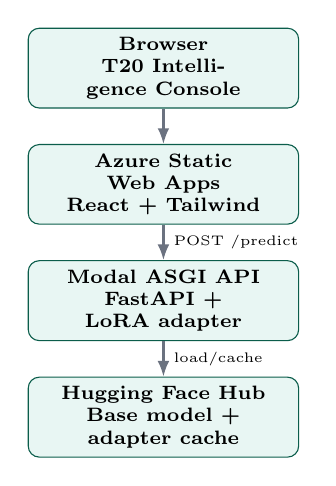
\begin{tikzpicture}[
    node distance=0.45cm,
    box/.style={draw=DeepGreen, fill=PaleGreen, rounded corners=4pt, text width=3.2cm, minimum height=0.85cm, align=center, font=\scriptsize\bfseries},
    arrow/.style={-{Latex[length=2mm]}, thick, draw=MidGrey}
  ]
    \node[box] (browser) {Browser\\T20 Intelligence Console};
    \node[box, below=of browser] (azure) {Azure Static Web Apps\\React + Tailwind};
    \node[box, below=of azure] (modal) {Modal ASGI API\\FastAPI + LoRA adapter};
    \node[box, below=of modal] (hf) {Hugging Face Hub\\Base model + adapter cache};
    \draw[arrow] (browser) -- (azure);
    \draw[arrow] (azure) -- node[right, font=\tiny]{POST /predict} (modal);
    \draw[arrow] (modal) -- node[right, font=\tiny]{load/cache} (hf);
  \end{tikzpicture}

  \vspace{0.25cm}
  \small\url{https://mango-ocean-00260de00.7.azurestaticapps.net/}
\end{columns}
\note{The deployment proves the work is not just a notebook result. The same stack can serve small-LLM prediction products in other sports contexts.}
\end{frame}

% =================================================
% Slide 15
% =================================================
\begin{frame}{References (Selected)}
\scriptsize
\begin{columns}[T,onlytextwidth]
  \column{0.49\textwidth}
  \begin{enumerate}
    \item Vaswani et al. (2017). \textit{Attention Is All You Need}.
    \item Brown et al. (2020). \textit{Language Models are Few-Shot Learners}.
    \item Touvron et al. (2023). \textit{LLaMA: Open and Efficient Foundation Language Models}.
    \item Hu et al. (2022). \textit{LoRA: Low-Rank Adaptation of Large Language Models}.
    \item Dettmers et al. (2023). \textit{QLoRA: Efficient Finetuning of Quantized LLMs}.
    \item Hegselmann et al. (2023). \textit{TabLLM: Few-shot Classification of Tabular Data with LLMs}.
  \end{enumerate}

  \column{0.49\textwidth}
  \begin{enumerate}
    \setcounter{enumi}{6}
    \item Gruver et al. (2023). \textit{Large Language Models are Zero-Shot Time Series Forecasters}.
    \item Huckerby et al. (2024). \textit{Leveraging LLMs for Football Match Outcome Prediction}.
    \item Duckworth and Lewis (1998). \textit{A Fair Method for Resetting Targets}.
    \item Bailey and Clarke (2004). \textit{Predicting Match Outcome in ODI Cricket}.
    \item Cricsheet (2024). \textit{A Cricketing Archive}.
  \end{enumerate}
\end{columns}

\vspace{0.35cm}
\begin{center}
\small Full bibliography appears in the thesis reference list.\\[0.15cm]
\Large\textbf{Thank you. Questions?}
\end{center}
\note{Full bibliography is in the thesis. These are the works most relevant to the methods and empirical claims.}
\end{frame}

\end{document}
\documentclass[aspectratio=169,10pt]{beamer}

% -----------------------------------------------------------------------------
% MSc Viva Presentation
% Generated from viva/presentation_plan.md
% -----------------------------------------------------------------------------

\usetheme{Madrid}
\usecolortheme{default}
\setbeamertemplate{navigation symbols}{}
\setbeamertemplate{caption}[numbered]
\setbeamertemplate{footline}[frame number]

\usepackage[T1]{fontenc}
\usepackage{lmodern}
\usepackage{booktabs}
\usepackage{array}
\usepackage{tabularx}
\usepackage{graphicx}
\usepackage{tikz}
\usepackage{amsmath}
\usepackage{hyperref}
\usepackage{ragged2e}
\usetikzlibrary{arrows.meta,positioning,shapes.geometric,fit,calc}

\graphicspath{{../thesis/figures/}}

\definecolor{primary}{HTML}{1F4E79}
\definecolor{accent}{HTML}{2C7A7B}
\definecolor{warn}{HTML}{B7791F}
\definecolor{good}{HTML}{2F855A}
\definecolor{bad}{HTML}{C53030}
\definecolor{softblue}{HTML}{EAF3FB}
\definecolor{softgreen}{HTML}{EAF7F1}
\definecolor{softamber}{HTML}{FFF6E5}
\definecolor{softgray}{HTML}{F3F4F6}

\setbeamercolor{structure}{fg=primary}
\setbeamercolor{frametitle}{bg=primary,fg=white}
\setbeamercolor{title}{fg=primary}
\setbeamercolor{block title}{bg=primary,fg=white}
\setbeamercolor{block body}{bg=softgray,fg=black}

\newcommand{\smallcaps}[1]{\textsc{#1}}
\newcommand{\metric}[3]{%
  \begin{tikzpicture}[baseline=(m.base)]
    \node[draw=#1, fill=#1!10, rounded corners=2pt, inner xsep=5pt, inner ysep=3pt] (m)
      {\textcolor{#1}{\textbf{#2}}\;{\scriptsize #3}};
  \end{tikzpicture}%
}
\newcommand{\pill}[2]{%
  \tikz[baseline=(p.base)]\node[fill=#1!12, draw=#1!65, rounded corners=7pt, inner xsep=6pt, inner ysep=2pt] (p) {\scriptsize #2};%
}
\newcommand{\tick}{\textcolor{good}{\textbf{Yes}}}
\newcommand{\cross}{\textcolor{bad}{\textbf{No}}}

\title[LLM Fine-Tuning for T20 Score Prediction]{Context-Aware Fine-Tuning of Large Language Models\\for First-Innings Score Prediction in T20 Cricket}
\subtitle{MSc Viva Presentation \textbar{} MSc DSA 055}
\author[Damith T. A. R. Ratnayaka]{Damith Tilanka Abewardana Ranasingha Ratnayaka}
\institute[USJ]{University of Sri Jayewardenepura\\Supervisor: Dr. Rajitha M. Silva}
\date{June 2026}

\begin{document}

% -----------------------------------------------------------------------------
\begin{frame}
  \titlepage
  \vspace{-0.4cm}
  \begin{center}
    \pill{accent}{Data source: Cricsheet ball-by-ball T20 JSON archive}
    \hspace{0.4em}
    \pill{primary}{Model: Llama 3.2-3B + QLoRA}
  \end{center}
\end{frame}

% -----------------------------------------------------------------------------
\begin{frame}{Motivation \& Significance}
\begin{columns}[T,onlytextwidth]
\column{0.48\textwidth}
\begin{block}{Why T20 Score Prediction Matters}
\begin{itemize}\setlength\itemsep{0.45em}
  \item T20 is short, high-variance, and commercially dominant.
  \item Live forecasts support broadcast graphics, fantasy products, betting markets, and team strategy.
  \item Useful prediction must integrate venue, phase, momentum, wickets, and batting depth.
\end{itemize}
\end{block}

\column{0.48\textwidth}
\begin{block}{Why LLMs Are Worth Testing}
\begin{itemize}\setlength\itemsep{0.45em}
  \item Conventional models usually consume flat numeric vectors.
  \item Analysts reason in rich natural-language context.
  \item LLMs can learn from structured text prompts, but cricket forecasting is largely unexplored.
\end{itemize}
\end{block}
\end{columns}

\vspace{0.45cm}
\begin{center}
\begin{tikzpicture}[node distance=0.8cm]
\node[draw=primary, fill=softblue, rounded corners, minimum width=4.0cm, minimum height=0.8cm] (vec) {Numeric vector};
\node[draw=accent, fill=softgreen, rounded corners, right=1.2cm of vec, minimum width=6.0cm, minimum height=0.8cm] (lang) {Natural-language match state};
\draw[-{Latex[length=2mm]}, thick] (vec) -- node[above, font=\scriptsize] {adds semantics} (lang);
\end{tikzpicture}
\end{center}
\end{frame}

% -----------------------------------------------------------------------------
\begin{frame}{Research Objectives \& Scope}
\small
\begin{tabularx}{\textwidth}{@{}>{\bfseries}p{0.9cm}X>{\bfseries}p{0.9cm}X@{}}
\toprule
RO1 & Construct temporal T20 state dataset with engineered RBSS. & RO2 & Design natural-language prompt--completion corpus. \\
RO3 & Establish zero-shot Llama 3.2-3B baseline. & RO4 & QLoRA fine-tune Llama 3.2-3B and evaluate gain. \\
RO5 & Compare minimum-validation-loss vs. final checkpoint. & RO6 & Evaluate GPT-4.1-nano zero-shot as frontier reference. \\
\bottomrule
\end{tabularx}

\vspace{0.55cm}
\begin{columns}[T,onlytextwidth]
\column{0.48\textwidth}
\begin{block}{In Scope}
\pill{good}{International men's T20}\quad
\pill{good}{First innings}\quad
\pill{good}{Two-over snapshots}\quad
\pill{good}{QLoRA fine-tuning}
\end{block}
\column{0.48\textwidth}
\begin{block}{Out of Scope}
\pill{warn}{Domestic leagues}\quad
\pill{warn}{Second-innings chase}\quad
\pill{warn}{Full fine-tuning}\quad
\pill{warn}{Uncertainty intervals}
\end{block}
\end{columns}
\end{frame}

% -----------------------------------------------------------------------------
\begin{frame}{Literature Review (1): Themes \& Trajectory}
\small
\begin{columns}[T,onlytextwidth]
\column{0.49\textwidth}
\begin{block}{Statistical Cricket Models}
\begin{itemize}\setlength\itemsep{0.25em}
  \item DLS/Stern: resource allocation.
  \item Markov models: ball-outcome transitions.
  \item Limitation: hand-crafted state assumptions.
\end{itemize}
\end{block}
\begin{block}{Machine Learning Cricket Models}
\begin{itemize}\setlength\itemsep{0.25em}
  \item Regression, random forests, SVMs, neural nets.
  \item Wickets and team strength are predictive.
  \item Limitation: numeric-vector representation.
\end{itemize}
\end{block}

\column{0.49\textwidth}
\begin{block}{LLM Foundations}
\begin{itemize}\setlength\itemsep{0.25em}
  \item Transformers enable scalable sequence modelling.
  \item Llama provides open decoder-only models.
  \item LoRA/QLoRA enables resource-efficient adaptation.
\end{itemize}
\end{block}
\begin{block}{LLMs for Structured Forecasting}
\begin{itemize}\setlength\itemsep{0.25em}
  \item TabLLM: tabular records as text.
  \item LLMs as time-series forecasters.
  \item Sports LLM work is emerging but limited.
\end{itemize}
\end{block}
\end{columns}
\end{frame}

% -----------------------------------------------------------------------------
\begin{frame}{Literature Review (2): Gap \& Contribution Map}
\scriptsize
\begin{tabularx}{\textwidth}{@{}lCCCC@{}}
\toprule
\textbf{Study / Stream} & \textbf{T20 prompt} & \textbf{RBSS-like feature} & \textbf{Small FT vs frontier} & \textbf{PEFT checkpoint} \\
\midrule
Perera--Swartz / Markov cricket & \cross & \cross & \cross & \cross \\
Kampakis--Thomas / ML cricket & \cross & \cross & \cross & \cross \\
Hegselmann / TabLLM & \cross & \cross & \cross & \cross \\
Huckerby / LLM sports & \cross & \cross & Partial & \cross \\
\rowcolor{softgreen}\textbf{This thesis} & \tick & \tick & \tick & \tick \\
\bottomrule
\end{tabularx}

\vspace{0.5cm}
\begin{block}{Research Gap}
No prior work combines a natural-language T20 match-state prompt, a batting-depth feature, QLoRA fine-tuning of a compact open-source LLM, and a head-to-head benchmark against a frontier zero-shot model.
\end{block}
\end{frame}

% -----------------------------------------------------------------------------
\begin{frame}{Methodology Overview}
\small
\begin{center}
\begin{tikzpicture}[
  box/.style={draw=primary, fill=softblue, rounded corners=2pt, minimum width=2.25cm, minimum height=1.0cm, align=center, font=\scriptsize},
  arrow/.style={-{Latex[length=2mm]}, thick, primary}
]
\node[box] (raw) {Cricsheet JSON\\3,113 files};
\node[box, right=0.35cm of raw] (filter) {Filter + venue\\normalisation\\2,895 matches};
\node[box, right=0.35cm of filter] (feat) {Feature\\engineering\\16 features};
\node[box, right=0.35cm of feat] (prompt) {Prompt corpus\\28,950 rows};
\node[box, right=0.35cm of prompt] (train) {QLoRA\\fine-tune};
\node[box, right=0.35cm of train] (eval) {Evaluation\\3 conditions};
\draw[arrow] (raw) -- (filter);
\draw[arrow] (filter) -- (feat);
\draw[arrow] (feat) -- (prompt);
\draw[arrow] (prompt) -- (train);
\draw[arrow] (train) -- (eval);
\end{tikzpicture}
\end{center}

\vspace{0.35cm}
\begin{columns}[T,onlytextwidth]
\column{0.33\textwidth}
\metric{primary}{236}{normalised venues}
\column{0.33\textwidth}
\metric{accent}{10}{snapshots per innings}
\column{0.33\textwidth}
\metric{good}{00be3f3f}{HF adapter revision}
\end{columns}

\vspace{0.45cm}
\begin{alertblock}{Key control}
Temporal splitting is applied before modelling to prevent future-match leakage and simulate real deployment.
\end{alertblock}
\end{frame}

% -----------------------------------------------------------------------------
\begin{frame}{Feature Engineering \& RBSS}
\small
\begin{columns}[T,onlytextwidth]
\column{0.48\textwidth}
\begin{block}{Snapshot Feature Groups}
\begin{itemize}\setlength\itemsep{0.35em}
  \item \textbf{State:} overs, balls, runs, wickets, run rate.
  \item \textbf{Recent form:} last-2-over runs, dots, boundaries.
  \item \textbf{Phase:} powerplay completed.
  \item \textbf{Venue:} historical par score at 52nd percentile.
  \item \textbf{Line-up:} Remaining Batting Strength Score.
\end{itemize}
\end{block}

\begin{center}
\begin{tikzpicture}[node distance=0.35cm]
\node[draw=accent, fill=softgreen, rounded corners, align=center, minimum width=5.1cm] (a) {Raw deliveries};
\node[draw=accent, fill=softgreen, rounded corners, align=center, below=of a, minimum width=5.1cm] (b) {Two-over sections};
\node[draw=accent, fill=softgreen, rounded corners, align=center, below=of b, minimum width=5.1cm] (c) {Prompt-ready features};
\draw[-{Latex[length=2mm]}] (a) -- (b);
\draw[-{Latex[length=2mm]}] (b) -- (c);
\end{tikzpicture}
\end{center}

\column{0.48\textwidth}
\begin{block}{RBSS Formula}
\[
\mathrm{RBSS}=\sum_{p\in \mathcal{R}} w(\mathrm{class}(p))
\]
\vspace{-0.3cm}
\begin{tabular}{@{}lr@{}}
\toprule
Role & Weight \\
\midrule
Batter & 1.00 \\
All-rounder & 0.80 \\
Utility player & 0.65 \\
Insufficient data & 0.45 \\
Bowler & 0.30 \\
\bottomrule
\end{tabular}
\end{block}

\begin{exampleblock}{Worked Example}
$1(1.00)+2(0.80)+1(0.65)+3(0.30)=\mathbf{4.15}$
\end{exampleblock}
\end{columns}
\end{frame}

% -----------------------------------------------------------------------------
\begin{frame}[fragile]{Prompt Schema \& Model Architecture}
\scriptsize
\begin{columns}[T,onlytextwidth]
\column{0.47\textwidth}
\begin{block}{Prompt Fragment}
\begin{verbatim}
Match type: T20
Venue: {venue}
Venue par score: {par_score}
Batting team: {team}
Overs completed: {overs}
Runs scored: {runs}
Wickets lost: {wickets}
Current run rate: {run_rate}
Runs in last 2 overs: {recent_runs}
Powerplay completed: {Yes|No}
Remaining Batting Strength Score: {RBSS}
Final 1st innings score:
\end{verbatim}
\end{block}

\column{0.50\textwidth}
\begin{block}{QLoRA Configuration}
\begin{tabularx}{\textwidth}{@{}lX@{}}
\toprule
Base model & Llama 3.2-3B \\
Quantisation & 4-bit NF4 + double quantisation \\
LoRA rank / alpha & $r=16$, $\alpha=32$ \\
Target modules & \texttt{q/k/v/o\_proj} \\
Dropout & 0.1 \\
Training & 1 epoch, lr $2\times10^{-4}$, effective batch 8 \\
Hardware & Kaggle NVIDIA T4, fp16 \\
\bottomrule
\end{tabularx}
\end{block}

\vspace{0.2cm}
\metric{primary}{148}{max prompt tokens}\quad
\metric{accent}{256}{max sequence length}\quad
\metric{good}{1.856}{min eval loss at step 800}
\end{columns}
\end{frame}

% -----------------------------------------------------------------------------
\begin{frame}{Data, Splits \& Tools}
\small
\begin{columns}[T,onlytextwidth]
\column{0.55\textwidth}
\begin{block}{Strict Temporal Split}
\begin{tabularx}{\textwidth}{@{}lXrr@{}}
\toprule
Split & Date range & Matches & Rows \\
\midrule
Train & Up to 2024-12-31 & 2,408 & 24,080 \\
Validation & 2025-01-01 to 2025-06-30 & 237 & 2,370 \\
Test & 2025-07-01 onward & 250 & 2,500 \\
\bottomrule
\end{tabularx}
\end{block}
\begin{alertblock}{Evaluation hygiene}
Temporal ordering prevents training on future match states and mirrors deployment on unseen matches.
\end{alertblock}

\column{0.42\textwidth}
\begin{block}{Tool Stack}
\pill{primary}{Pydantic v2}\quad \pill{primary}{SQLite}\quad \pill{primary}{fuzzywuzzy}
\vspace{0.25cm}

\pill{accent}{HF Datasets}\quad \pill{accent}{PEFT}\quad \pill{accent}{TRL}\quad \pill{accent}{BitsAndBytes}
\vspace{0.25cm}

\pill{good}{W\&B}\quad \pill{good}{LiteLLM}\quad \pill{good}{Modal}\quad \pill{good}{Gradio}
\vspace{0.25cm}

\pill{warn}{React/Vite}\quad \pill{warn}{Azure SWA}\quad \pill{warn}{Bicep + OIDC}
\end{block}
\end{columns}
\end{frame}

% -----------------------------------------------------------------------------
\begin{frame}{Results: Headline Comparison}
\small
\begin{columns}[T,onlytextwidth]
\column{0.56\textwidth}
\begin{block}{Mean Absolute Error (runs)}
\begin{tikzpicture}[x=0.95cm,y=0.065cm]
\draw[->] (0,0) -- (0,78) node[above, font=\scriptsize] {MAE};
\draw[->] (0,0) -- (7.2,0);
\foreach \y in {0,20,40,60} {\draw (-0.08,\y) -- (0.08,\y) node[left=0.12cm, font=\scriptsize] {\y};}
\fill[bad!75] (0.8,0) rectangle (1.8,71.31);
\fill[warn!75] (3.0,0) rectangle (4.0,30.02);
\fill[good!75] (5.2,0) rectangle (6.2,16.51);
\node[font=\scriptsize, align=center] at (1.3,-6) {Llama\\zero-shot};
\node[font=\scriptsize, align=center] at (3.5,-6) {GPT-4.1-nano\\zero-shot};
\node[font=\scriptsize, align=center] at (5.7,-6) {Llama\\fine-tuned};
\node[font=\scriptsize] at (1.3,74.5) {71.31};
\node[font=\scriptsize] at (3.5,33.5) {30.02};
\node[font=\scriptsize] at (5.7,20.0) {16.51};
\end{tikzpicture}
\end{block}

\column{0.41\textwidth}
\begin{block}{Cross-condition Metrics}
\scriptsize
\begin{tabularx}{\textwidth}{@{}Xrrr@{}}
\toprule
Model & $n$ & MAE & $R^2$ \\
\midrule
Llama zero-shot & 200 & 71.31 & -317.4\% \\
GPT-4.1-nano ZS & 200 & 30.02 & 14.0\% \\
\textbf{Llama fine-tuned} & \textbf{500} & \textbf{16.51} & \textbf{68.3\%} \\
\bottomrule
\end{tabularx}
\end{block}

\metric{good}{76.8\%}{MAE reduction vs. Llama ZS}
\vspace{0.15cm}

\metric{good}{45.0\%}{MAE reduction vs. GPT-4.1-nano}
\vspace{0.15cm}

\metric{good}{+54.3 pp}{$R^2$ vs. GPT-4.1-nano}
\end{columns}
\end{frame}

% -----------------------------------------------------------------------------
\begin{frame}{Discussion: Why Fine-Tuning Wins}
\small
\begin{columns}[T,onlytextwidth]
\column{0.48\textwidth}
\begin{block}{Interpretation}
\begin{itemize}\setlength\itemsep{0.4em}
  \item General pre-training contains cricket prose, not the conditional map $P(\mathrm{final}\mid\mathrm{state})$.
  \item Fine-tuning supplies thousands of labelled prompt--score pairs.
  \item GPT-4.1-nano often underestimates early-innings states by applying near-linear projection.
  \item Venue par score and RBSS enrich the prompt beyond raw score and wickets.
\end{itemize}
\end{block}
\begin{exampleblock}{Checkpoint selection}
At $n=500$, the step-800 checkpoint beats the final checkpoint on MAE, MSE, and $R^2$.
\end{exampleblock}

\column{0.48\textwidth}
\begin{block}{Validation Loss Evidence}
\includegraphics[width=\textwidth,height=0.56\textheight,keepaspectratio]{wandb_eval_loss.png}
\end{block}
\vspace{-0.1cm}
\centering
\metric{accent}{Step 800}{minimum eval loss = 1.856}
\end{columns}
\end{frame}

% -----------------------------------------------------------------------------
\begin{frame}{Limitations}
\small
\begin{columns}[T,onlytextwidth]
\column{0.48\textwidth}
\begin{block}{Scope Limitations}
\begin{itemize}\setlength\itemsep{0.35em}
  \item International men's T20 only.
  \item Domestic leagues such as IPL, BBL, PSL excluded.
  \item First innings only; chase prediction not modelled.
  \item GPT-4.1-nano evaluated at $n=200$ due to API cost.
\end{itemize}
\end{block}

\column{0.48\textwidth}
\begin{block}{Methodological Limitations}
\begin{itemize}\setlength\itemsep{0.35em}
  \item Single fine-tuning run; no multi-seed estimate.
  \item Base model limited to 3B parameters.
  \item Validation loss computed on first 50 validation rows.
  \item Point predictions only; no calibrated uncertainty.
  \item Regex fallback-to-zero inflates zero-shot Llama error.
\end{itemize}
\end{block}
\end{columns}

\vspace{0.35cm}
\begin{alertblock}{Defence position}
These are bounded by compute and cost constraints; they define the next experiments rather than invalidating the observed effect size.
\end{alertblock}
\end{frame}

% -----------------------------------------------------------------------------
\begin{frame}{Conclusions \& Future Work}
\small
\begin{columns}[T,onlytextwidth]
\column{0.48\textwidth}
\begin{block}{Conclusions}
\begin{enumerate}\setlength\itemsep{0.45em}
  \item Fine-tuning transforms zero-shot Llama from unusable to competitive.
  \item A small fine-tuned open-source model beats zero-shot GPT-4.1-nano on this task.
  \item Minimum-validation-loss checkpoint selection generalises marginally better at scale.
\end{enumerate}
\end{block}

\column{0.48\textwidth}
\begin{block}{Future Work}
\pill{primary}{Domestic T20 leagues}\quad
\pill{primary}{7B/8B/70B models}
\vspace{0.25cm}

\pill{accent}{Second innings}\quad
\pill{accent}{Live data feeds}
\vspace{0.25cm}

\pill{good}{Prediction intervals}\quad
\pill{good}{Feature ablation}
\end{block}
\end{columns}

\vspace{0.35cm}
\begin{exampleblock}{Main claim}
Domain-specific QLoRA fine-tuning can matter more than frontier-model scale for structured numerical sports forecasting.
\end{exampleblock}
\end{frame}

% -----------------------------------------------------------------------------
\begin{frame}{Practical Implications}
\small
\begin{columns}[T,onlytextwidth]
\column{0.46\textwidth}
\begin{block}{For Cricket Analytics Teams}
\begin{itemize}\setlength\itemsep{0.4em}
  \item Curate labelled ball-by-ball data before buying frontier APIs.
  \item Fine-tune compact open-source models in-house.
  \item Use point forecasts for trend analysis, not high-stakes settlement.
\end{itemize}
\end{block}
\begin{block}{Operational Latency}
\metric{warn}{30 s}{cold start}\quad
\metric{good}{2 s}{warm response}
\end{block}

\column{0.50\textwidth}
\begin{center}
\begin{tikzpicture}[
  node distance=0.55cm,
  box/.style={draw=primary, fill=softblue, rounded corners=2pt, minimum width=4.8cm, minimum height=0.65cm, align=center, font=\scriptsize},
  arrow/.style={-{Latex[length=2mm]}, thick, primary}
]
\node[box] (browser) {Browser / React dashboard};
\node[box, below=of browser] (azure) {Azure Static Web Apps};
\node[box, below=of azure] (modal) {Modal FastAPI + warm GPU service};
\node[box, below=of modal] (model) {HF Hub: Llama 3.2-3B + LoRA adapter};
\draw[arrow] (browser) -- (azure);
\draw[arrow] (azure) -- (modal);
\draw[arrow] (modal) -- (model);
\end{tikzpicture}
\end{center}
\vspace{0.15cm}
\centering
\pill{accent}{Gradio prototype}\quad \pill{accent}{React/Vite UI}\quad \pill{accent}{Bicep + GitHub Actions OIDC}
\end{columns}
\end{frame}

% -----------------------------------------------------------------------------
\begin{frame}{References (Selected)}
\scriptsize
\begin{columns}[T,onlytextwidth]
\column{0.48\textwidth}
\begin{enumerate}\setlength\itemsep{0.25em}
  \item Vaswani et al. (2017), \textit{Attention Is All You Need}.
  \item Brown et al. (2020), \textit{Language Models are Few-Shot Learners}.
  \item Touvron et al. (2023), \textit{LLaMA}.
  \item Hu et al. (2022), \textit{LoRA}.
  \item Dettmers et al. (2023), \textit{QLoRA}.
  \item Hegselmann et al. (2023), \textit{TabLLM}.
\end{enumerate}
\column{0.48\textwidth}
\begin{enumerate}\setcounter{enumi}{6}\setlength\itemsep{0.25em}
  \item Gruver et al. (2023), \textit{LLMs as Time-Series Forecasters}.
  \item Huckerby et al. (2024), LLMs for football match prediction.
  \item Duckworth and Lewis (1998), DLS resource method.
  \item Bailey and Clarke (2004), cricket outcome prediction.
  \item Cricsheet (2024), cricket ball-by-ball archive.
\end{enumerate}
\end{columns}

\vspace{0.5cm}
\begin{center}
\Large Thank you. Questions?
\end{center}
\end{frame}

\end{document}
